%************************************************
\chapter{Computer Assisted Pronunciation Training}\label{ch:capt}
%************************************************

\section{PB}

1 Sistemas de Reconhecimento de Pron\'uncia

Um reconhecedor de pron\'uncia nada mais \'e do que um reconhecedor de fala
voltado a uma tarefa espec\'ifica, qual seja: compreender e analisar a
pron\'uncia de um aprendiz. Como j\'a discutido, um reconhecedor de fala \'e
um sistema computacional que recebe como entrada um sinal ac\'ustico de
fala e fornece como sa\'ida a transcri\c{c}\~ao textual da informa\c{c}\~ao contida na
fala (Rabiner \& Schafer, 2007).

Reconhecedores de pron\'uncia s\~ao ferramentas de interesse, especialmente,
na \'area de Computer-Assisted Language Learning (CALL), sub\'area da
Lingu\'istica Aplicada que se dedica ao estudo da utiliza\c{c}\~ao de
computadores para aprendizagem de l\'ingua (Beatty, 2002). Os sistemas de
CALL que auxiliam no aprendizado ou na pr\'atica da pron\'uncia de outras
l\'inguas s\~ao os chamados Computer-Assisted Pronunciation Training (CAPT).
Tais sistemas s\~ao \'utes, especialmente, por quatro motivos: (i) sua
difus\~ao: basta ter acesso a um computador para utiliz\'a-los; (ii) sua
capacidade de fornecer feedback individual - nas salas de aula
tradicionais, dado o tempo, nem sempre \'e poss\'ivel ao professor corrigir
verbatim a pron\'uncia de cada aluno; (iii) seu baixo custo - tais
tecnologias possuem baixo custo, se comparadas ao gasto com um curso de
pron\'uncia; (iv) sua possibilidade de propiciar autoestudo ass\'incrono - o
aluno pode treinar sua pron\'uncia onde e quando quiser, independentemente
de um lugar ou hor\'ario espec\'ifico (Witt, 1999).

Sistemas de CAPT, em geral, tentam agregar os  seguintes  componentes:

listas de pron\'uncia, material expositivo com informa\c{c}\~oes ac\'ustico-
articulat\'orias de cada som, tutoriais e exerc\'icios de transcri\c{c}\~ao,
atividade para pr\'atica e avalia\c{c}\~ao de pron\'uncia. Dois desses sistemas,
notadamente, Accent Master e Macmillan Education Sounds s\~ao analisados a
seguir.

O Accent Master \'e um software pago, que busca ensinar a pron\'uncia do AmE
a partir de atividades, exerc\'icios, jogos, v\'ideos expositivos e
anima\c{c}\~oes. A parte de exposi\c{c}\~ao e ensino de pron\'uncia do software \'e bem
completa e possui explica\c{c}\~oes detalhadas de como se produz cada fone do
AmE, al\'em de v\'ideos e anima\c{c}\~oes da posi\c{c}\~ao dos \'org\~aos do aparelho
fonador. O software possui vers\~oes espec\'ificas para a l\'ingua nativa do
aprendiz (atualmente, h\'a suporte para 21 l\'inguas, incluindo o PB). As
vers\~oes espec\'ificas compreendem uma descri\c{c}\~ao dos sons da l\'ingua nativa,
bem como instru\c{c}\~oes sobre quais aspectos de pron\'uncia devem ser focados.
Por\'em o Accent Master n\~ao possui um sistema de reconhecimento de fala
built-in. O treinamento de pron\'uncia d\'a-se da seguinte forma: primeiro,
o aprendiz ouve uma palavra em ingl\^es, tenta repeti-la, ent\~ao, o
software plota no monitor o oscilograma da palavra ouvida e de sua
tentativa, e cabe ao pr\'oprio aprendiz comparar se a realiza\c{c}\~ao foi
similar ou n\~ao. No entanto, deixar ao aprendiz a an\'alise do oscilograma
n\~ao constitui uma boa solu\c{c}\~ao, pois, mesmo considerando a enuncia\c{c}\~ao de
uma mesma palavra, a forma de um oscilograma \'e bastante vari\'avel e
depende de caracter\'isticas do aparelho fonador (Johnson \& Mullenix,
1997). Al\'em disso, trabalhos anteriores a respeito de Sistemas de CALL
j\'a questionaram o valor pedag\'ogico deste tipo de atividade (Neri et al.,
2008). A Figura 10 cont\'em algumas telas da interface do software Accent
Master.

                         [pic]  [pic]  [pic]

           Figura 10: Telas da interface do Accent Master.

O Macmillan Education Sounds: The Pronunciation App \'e um aplicativo de
ensino de pron\'uncia do ingl\^es para iPhone, iPad e Android. Trata-se de
um software com uso gratuito limitado e compras in-app, que foi
desenvolvido para treinamento da pron\'uncia tanto do AmE, quanto do BrE.
O app possui exerc\'icios de reading, writing e listening para treinar a
transcri\c{c}\~ao fon\'etica das palavras do ingl\^es. No entanto, n\~ao h\'a nenhum
tipo de introdu\c{c}\~ao à fonologia ou fon\'etica do ingl\^es, de modo que se
pressup\~oe que o usu\'ario j\'a tenha dom\'inio do Alfabeto Fon\'etico
Internacional (AFI) e das conven\c{c}\~oes de transcri\c{c}\~ao das palavras do
ingl\^es. Sendo assim, a utiliza\c{c}\~ao do software acaba por restringir-se a
aprendizes intermedi\'arios e avan\c{c}ados de ingl\^es que saibam utilizar o
Alfabeto Fon\'etico Internacional. O exerc\'icio de pron\'uncia \'e composto por
um dicion\'ario, que cont\'em o \'audio das palavras e que possibilita ao
aprendiz gravar sua pr\'opria fala e comparar com o \'audio existente no
dicion\'ario. O app n\~ao possui reconhecimento de fala e, por conseguinte,
n\~ao h\'a nenhum tipo de avalia\c{c}\~ao ou feedback da pron\'uncia do usu\'ario. A
Figura 11 cont\'em exemplos da interface do software gratuito.

                         [pic]  [pic]  [pic]

Figura 11: Telas da interface do software Macmillan Education - Sounds.

\section{English}

Many papers have confirmed the importance of feedback for adequate learning in second language
acquisition. Negative feedback has been investigated by (XXXXX) and positive feedback by (XXXXX).
For \ac{CAPT} systems the feedback to the user may be provided by many media: text, voice or video.

Definitely, the more complex and informative form of feedback is through video. \citeauthor{Badin2010} \citep{Badin2010}
developed a 3D talking head, that is able to display the articulation in an augmented mode,
by showing all major speech articulators, including those usually hidden such as the tongue or the velum. The talking
was called OroFacial Clone, and an example of its display can be found in \autoref{fig:badin-orofacial-clone}.

\begin{figure}[!htb]
        \myfloatalign
        {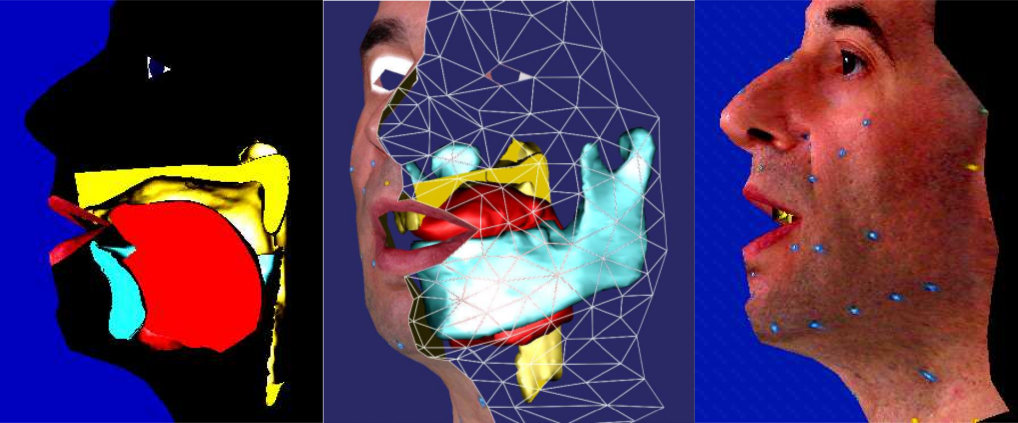
\includegraphics[width=.66\linewidth]{gfx/badin-orofacial-clone.png}}
        \caption{Example of the OroFacial Clone display, from \citeauthor{Badin2010} \citep{Badin2010}.}
        \label{fig:badin-orofacial-clone}
\end{figure}

The model is based on acustic-to-articulatory inversion and was built upon estimating speech articulators' 
movement from \ac{MRI}, \ac{CT} and video data. As one can imagine, building such a model is a very expensive task, which 
requires not only \ac{CG} and speech processing expertise, but also access to high-priced medical devices, such as 
\ac{MRI} scanners and tomographs. 

Part of this system was evaluated by \citeauthor{Wang2014} \citep{Wang2014} in a \ac{CAPT} context, by testing the
performance of Chinese learners of French. The aim of the test was to analyse the performance of the learners in the production 
and perception of the French vowels [\textipa{\o}] and [\textipa{\oe}], that do not exist in Chinese. The authors found that the 
students exposed to audiovisual stimuli produced vowels that were closer to the correct ones than the subjects who had access only 
to the auditory stimuli. After training, the difference between the F1 of [\textipa{\o}] and [\textipa{\oe}] was $62$ Hz for the audio
group and $178$ Hz for the audiovisual group. Additionaly, the audiovisual group performed better in 
an [\textipa{\o}] and [\textipa{\oe}] perception test, the number of correct responses rose from 61\% to 68\% for the audio only
group, and from 50\% to 86\% for the audiovisual one.




%*****************************************
%*****************************************
%*****************************************
%*****************************************
%*****************************************
